%&pdflatex
\documentclass[mathserif]{beamer} %, handout
\usetheme[progressbar=foot]{metropolis}
\setbeamertemplate{caption*}[numbered]

\usepackage[utf8x]{inputenc}
\usepackage[T2A]{fontenc}
\usepackage[english,russian]{babel}

\usepackage{amssymb, amsmath, amsfonts, mathtools, mathrsfs}
\usepackage[normalem]{ulem} % for sout
\usepackage{comment}

\title{Математическая теория уравнения Больцмана. Обзор современных достижений}
\author{Рогозин Олег Анатольевич}
\institute{
    Вычислительный центр ФИЦ ИУ РАН
}
\date{}

\newcommand{\Kn}{\mathrm{Kn}}
\newcommand{\St}{\mathrm{St}}
\newcommand{\Ma}{\mathrm{Ma}}
\newcommand{\loc}{\mathrm{loc}}
\newcommand{\eqdef}{\overset{\mathrm{def}}{=}}
\newcommand{\dd}{\:d}%{\:\mathrm{d}}
\newcommand{\pder}[2][]{\partial_{#2}{#1}}
\newcommand{\pderdual}[2][]{\partial_{#2^2}{#1}}
\newcommand{\pderder}[2][]{\frac{\partial^2 #1}{\partial #2^2}}
\newcommand{\Pder}[2][]{\partial#1/\partial#2}
\newcommand{\dxi}{\dd\xi}
\newcommand{\OO}[1]{O(#1)}
\newcommand{\Set}[2]{\{\,{#1}:{#2}\,\}}
\newcommand{\xoverbrace}[2][\vphantom{\int}]{\overbrace{#1#2}}
\newcommand{\Cite}[2][]{\alert{\textsc{#2 #1}}}
\newcommand{\inner}[2]{\left\langle{#1},{#2}\right\rangle}

% use Russian tradition
\renewcommand{\phi}{\varphi}
\renewcommand{\epsilon}{\varepsilon}

\begin{document}

\frame{\titlepage}

\begin{frame}
    \frametitle{Актуальность}
    \begin{block}{Государственная премия СССР (1989)}
        \begin{itemize}
            \item Арсеньев Алексей Алексеевич\\ (1938--2013, МГУ)
            \item Бобылев Александр Васильевич\\ (род. 1947, ИПМ им. Келдыша)
            \item Веденяпин Виктор Валентинович\\ (род. 1949, ИПМ им. Келдыша)
            \item М\'{а}слова Нина Борисовна\\ (1939--1993, институт океанологии)
        \end{itemize}
        За математические методы исследования уравнения Больцмана
    \end{block}
\end{frame}

\begin{frame}
    \frametitle{Содержание}
    \linespread{0.8}
    \tableofcontents
\end{frame}

\section{Уравнение Больцмана}

\begin{frame}
    \frametitle{Функция распределения}
    Microscopic description (identical particles with Hamiltonian):
    \begin{equation*}
        H(x,\xi) = \frac12 \sum_{i=1}^{N}|\xi_i|^2 + \sum_{i\ne j} U(x_i - x_j).
    \end{equation*}
    Mesoscopic description: % минимальные предположения
    \begin{equation*}
        f(t,x,\xi): \mathbb{R}_+\times\Omega\times\mathbb{R}^d\mapsto\mathbb{R}_+
        \quad (\Omega\subset\mathbb{R}^d),
    \end{equation*}
    \begin{equation*}
        f(t,\cdot,\cdot) \in L^1_\loc(\Omega; L^1(\mathbb{R}^d)).
    \end{equation*}
    Macroscopic quantities: % часто более гладкие, чем ФР
    \begin{gather*}
        \rho = \int_{\mathbb{R}^d} f\dxi, \\
        v = \frac1\rho\int_{\mathbb{R}^d} \xi f\dxi, \\
        T = \frac1{d\rho}\int_{\mathbb{R}^d} \left(|\xi|^2 - |v|^2\right) f\dxi.
    \end{gather*}
\end{frame}

\begin{frame}
    \frametitle{Уравнение Больцмана}
    \begin{equation*}
        \pder[f]{t} + \xi\cdot\pder[f]{x} = Q(f,f).
    \end{equation*}

    \begin{itemize} % с точки зрения энтропии
        \item \(\xi\cdot\pder{x}\) "--- transport operator (conservative)
        \item \(Q(f,f)\) "--- collisional operator (dissipative)
    \end{itemize}

    \begin{gather*}
        Q(f,f)(t,x,\xi) \eqdef \int_{\mathbb{R}^d}\dxi_* \int_{S^{d-1}} \dd\sigma
        \overbrace{B(\xi-\xi_*,\sigma)}^\text{collisional kernel}
        \Big( \overbrace{f'f'_*}^\text{gain} - \overbrace{ff_*}^\text{loss} \Big), \\
        \xi' = \dfrac{\xi+\xi_*}2 + \dfrac{|\xi-\xi_*|}2\sigma, \quad
        \xi'_* = \dfrac{\xi+\xi_*}2 - \dfrac{|\xi-\xi_*|}2\sigma.
    \end{gather*}

\end{frame}

\begin{frame}
    \frametitle{Симметрии и H-теорема Больцмана}
    Weak formulation:
    \begin{equation*}
        \int_{\mathbb{R}^d} Q(f,f)\phi = \frac14 \int_{\mathbb{R}^d} Q(f,f) (\phi + \phi_* - \phi' - \phi'_*).
    \end{equation*}
    \pause
    Lyapunov functional or H-functional or negative entropy:
    \begin{equation*}
        H(f) \eqdef \int_{\Omega\times\mathbb{R}^d} f\log{f} \xrightarrow{t\to\infty} \min.
    \end{equation*}
    Entropy production functional:
    \begin{equation*}
        D(f) \eqdef -\int_{\mathbb{R}^d} Q\log{f} = \frac14\int_{\mathbb{R}^{2d}\times S^{d-1}}
        B\left( f'f'_* - ff_* \right) \log\frac{f'f'_*}{ff_*} \geq 0.
    \end{equation*}
    H-theorem:
    \begin{equation*}
        \pder[H]{t} = - \int_\Omega D.
    \end{equation*}
\end{frame}

\begin{frame}
    \frametitle{Классификация столкновительных ядер}
    \begin{gather*}
        U(r)\sim r^{1-s} \:\implies\: \sin^{d-1}\theta B(|\xi-\xi_*|,\cos\theta) \sim |\xi-\xi_*|^\gamma \theta^{-1-\nu}, \\
        \quad \gamma = \dfrac{s-5}{s-1}\in[-3,1), \quad \nu = \dfrac2{s-1}\in(0,2].
    \end{gather*}
    \begin{itemize}
        \item hard spheres: \(s=+\infty,\quad\gamma=1,\quad\nu=0 \quad\implies\quad B=|\bxi-\bxi_*|\)
        \item hard potentials: \(\gamma>0\)
        \item Maxwell: \(s=5,\quad\gamma=0,\quad\nu=\frac12\), \quad \Cite[1984]{Bobylev}\\
            {\footnotesize Бобылев Александр Васильевич (род. 1947, ИПМ им. Келдыша)}
        \item soft potentials: \(\gamma<0\)
        \item Coulomb: \(s=2,\quad\gamma=-3,\quad\nu=2\) \(\:\longrightarrow\:\) Landau equation,\\
            \Cite[1990]{Arsen'ev, Buryak}, \Cite[1998]{Villani} \\
            {\footnotesize Арсеньев Алексей Алексеевич (1938--2013, МГУ)}
    \end{itemize}
\end{frame}

\begin{frame}
    \frametitle{Вывод из уравнения Лиувилля}
    Boltzmann--Grad (low-density) limit: \[ Nr^{d-1}=\OO{1}, \quad N\to\infty \]\vspace{-20pt}
    \begin{itemize}
        \item \Cite[1958]{Grad}: correct limiting procedure for HS
        \item \Cite[1972]{Cercignani}: rigorous formulation (need \(\exists!\) theorems)
        \item \Cite[1975]{Lanford}: rigorous result for short times and HS
        \item \Cite[1986]{Illner, Pulvirenti}:\\ full result for rare cloud of gas expanding in the vacuum
        \item \Cite[1990]{Petrina, Gerasimenko}: first explicit estimates\\
            {\footnotesize Петрина Дмитрий Яковлевич (1934--2006)}
        \item \Cite[2013]{Gallagher, Saint-Raymond, Texier}:\\ recollisions, smooth positive hard cutoff potentials
        \item \Cite[2015]{Bodineau, Gallangher, Saint-Raymond}:\\ linear Boltzmann for \(t\ll\ln\ln N\)
        \item \Cite[2016]{...}: linearized Boltzmann for 2D and \(t\ll\sqrt[4]{\ln\ln N}\)
    \end{itemize}
%    We call pathological a trajectory such that
%        1) there exists a collision involving more than two particles
%        2) the collision is grazing
%        3) there are an infinite number of collisions in finite time so the dynamics cannot be defined globally.
\end{frame}

\section{Решение задачи Коши}
%%% Pierre-Louis Lions (Пьер-Луи Ли'онс)

\subsection{пространственно-однородная задача}

\begin{frame}
    \frametitle{Теория жёстких усечённых потенциалов}
    \Cite[1958]{Grad}: Grad's angular cutoff = short-range assumption
    \[ \int_{S^{d-1}} b\dd\sigma = |S^{d-2}|\int_0^\pi b(\cos\theta) \sin^{d-2}\theta\dd\theta < \infty \]
    Existence and uniqueness of \(\pder[f]{t} = Q(f,f)\) in \(L^1\) for \(\pder{t}\int|\xi|^2f=0\): \vspace{-20pt}
    \begin{itemize}
        \item \Cite[1933]{Carleman}, \Cite[1962]{Povzner}: hard spheres \\
        {\footnotesize Повзнер Александр Яковлевич (1915--2008)}
        \item \Cite[1955]{Morgenstern}: Maxwellian molecules
        \item \Cite[1972]{Arkeryd}: hard potentials
        \item \Cite[1999]{Mischler, Wennberg}: optimal result (\(f_0\in L^1_2\), \sout{\(L\log{L}\)})\!\!\!\!\!\!\!\!\!\!
        \[ L^1_q \eqdef \Set{f}{\int_{\mathbb{R}^d} f(1+|\xi|^q) < +\infty}. \]
        \item \Cite[1999]{Wennberg}: nonuniqueness result (increasing energy)
    \end{itemize}
\end{frame}

\begin{frame}
    \frametitle{Теория жёстких усечённых потенциалов}
    \begin{itemize}
        \item \Cite[1999]{Mischler, Wennberg}: moment bounds
        \[ \forall q\geq2: \sup_{t\geq t_0>0} \int_{\mathbb{R}^d} f_t (1+|\xi|^q) \]
        \item \Cite[1997]{Pulvirenti, Wennberg}: Maxwellian lower bound
        \[ \forall t_0>0, \exists K_0,A_0>0: f_{t>0}(\xi) \geq K_0\exp\left( -A_0 |\xi|^2\right) \]
        \item \Cite[2009]{Gamba, Panferov, Villani}: Maxwellian upper bound \!\!\!\!\!
        \[ f_0 \leq M_0(\xi) \implies f_t \leq M(\xi)\]
        \item \Cite[2004]{Mouhot, Villani}: regularization theory (gain term)
        \begin{gather*}
            \forall s\geq0,q\geq0,t_0>0,k>0 : f_{t\geq t_0} = f^S_t + f^R_t, \\
            \sup_{t\geq t_0} \|f^S_t\|_{H^s_q\cap L_2^1} < +\infty,
            \quad \|f^R_t\|_{L_k^1} = \OO{e^{-\lambda t}}
        \end{gather*}
    \end{itemize}
\end{frame}

\begin{frame}
    \frametitle{Теория мягких потенциалов}
    \begin{itemize}
        \item \Cite[1981]{Arkeryd}, \Cite[1997]{Goudon}: weak solutions (\(\gamma\geq-2\))
        \[ (\phi + \phi_* - \phi' - \phi'_*) \sim |z|^2 \]
        \item \Cite[1999]{Villani}: H-solutions (\(-4<\gamma<-2\))
        \begin{gather*}
            D(f) \geq \int_{\mathbb{R}^{2d}\times S^{d-1}} B(|z|, \sigma) \left(\sqrt{f'f'_*} - \sqrt{ff_*}\right)^2, \\
            \left| \int_{\mathbb{R}^d} Q(f,f)\phi \right| \leq \frac12
            \sqrt{ D(f) \int Bff_* (\phi + \phi_* - \phi' - \phi'_*)^2 }
        \end{gather*}
        \item Bad estimates on moments:
        \[ \forall q>2: \quad\int_{\mathbb{R}^d} f_t |\xi|^q < C(1+t) \]
    \end{itemize}
\end{frame}

\begin{frame}
    \frametitle{Теория неусечённых потенциалов}
    Nonintegrable angular singularity due to grazing collisions (\(\theta\to0\)):
    \[ \int_0^\pi b(\cos\theta)\sin^{d-2}\theta\dd\theta = +\infty \]
    \vspace{-20pt}
    \begin{itemize}
        \item \Cite[2000]{Alexandre, Desvillettes, Villani, Wennberg}:
        \begin{gather*}
            \text{collisional} \:\longrightarrow\: \text{diffusive--collisional} \\
            D(g,f) \eqdef -\int_{\mathbb{R}^d} Q(g,f)\log{f} \geq C_1\|\sqrt{f}\|^2_{H^\frac\nu2} - C_2\|f\|_{L^1_2}\|g\|_{L^1_2}, \\
            \implies Q \sim -(-\Delta)^\frac\nu2 % fractional Laplace operator
        \end{gather*}
        \item \Cite[2004]{Desvillettes, Wennberg}: Schwartz space \(\mathscr{S}\)
        \[ f \in L^\infty\left([t_0>0,+\infty); \mathscr{S}(\mathbb{R}^d)\right) \]
        \item \Cite[2009]{Desvillettes, Mouhot}: uniqueness
        \[ \forall\nu\in(0,2): \quad\exists! f_t\in W_q^{1,1} \]
    \end{itemize}
\end{frame}

\subsection{пространственно-неоднородная задача}

\begin{frame}
    \frametitle{Нелинейная теория возмущений}
    Near-equilibrium solutions:
    \[ \exists \alpha_1, \alpha_2, \lambda > 0 \quad \forall h\in L^2(M^{-1}):
        \|h_0\|<\alpha_1 \implies \|h_t\|<\alpha_2 e^{-\mu t}  \] \vspace{-10pt}
    \begin{itemize}
        \item \Cite[1964]{Grad}: local (\(t\in(0,T]\)) for hard cutoff
        \item \Cite[1974]{Ukai}, \Cite[1975]{Maslova, Firsov}: global (\(t\in(0,+\infty)\))\\
            {\footnotesize М\'{а}слова Нина Борисовна (1939--1993)}
        \item \Cite[1980]{Caflisch}: extension for weak solutions (\(\gamma>-2\))
        \item \Cite[2003]{Guo}: extension for H-solutions (\(\gamma>-3\))
        \item \Cite[2008]{Strain, Guo}: exponential decay of smooth \(h\) for soft
        \item \Cite[2011]{Gressman, Strain}: extension for non-cutoff in \(\mathbb{T}^d\)
        \item \Cite[2011]{Alexandre, Morimoto, Ukai, Xu, Yang}: in \(\mathbb{R}^d\)
        \begin{gather*}
            h_t = \OO{e^{-\lambda t}} \quad\text{for}\quad \gamma+\nu \geq0, \\
            h_t =\OO{t^{-\infty}} \quad\text{for}\quad \gamma+\nu <0.
        \end{gather*}
    \end{itemize}
\end{frame}

\begin{frame}
    \frametitle{Сглаживающие свойства оператора переноса}
    {\centering Velocity-averaging lemmas}
    % macroscopic observables enjoy some smoothness properties even when the distribution function itself does not
    \begin{equation*}
        f\in L^2_{t,x,\xi}, Q\in L^2_{t,x}(H_\xi^s) \implies
            \forall\phi\in C^\infty: \int_{\mathbb{R}^d} f\phi\in H_{t,x}^{\frac1{2(1+s)}}
    \end{equation*}
    \begin{itemize}
        \item \Cite[1984]{Agoshkov}: first compactness result \\
            {\footnotesize Агошков Валерий Иванович (р. 1946, ИВМ)}
        \item \Cite[1985]{Golse, Perthame, Sentis}:\\compact in \(L_\mathrm{loc}^p(\mathbb{R}^d)\) for \(p\in(1,\infty)\)
        \item \Cite[1988]{..., Lions}: bound in some Sobolev space
        \item \Cite[1998]{Lions}: optimal Sobolev space
        \item \Cite[2002]{Golse, Saint-Raymond}: extension to \(L^1\) case
    \end{itemize}
\end{frame}

\begin{frame}
    \frametitle{\(L^1\)-теория}
        \begin{columns}
    \begin{column}{0.2\textwidth}
       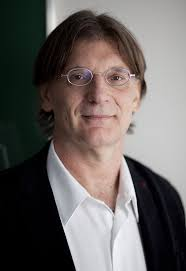
\includegraphics[width=1.4\textwidth]{../boltzmann_math/photos/lions}\\
       Pierre-Louis\\Lions\\(b. 1956)
    \end{column}
    \begin{column}{0.8\textwidth}
        \begin{itemize}
            \item \Cite[1989]{DiPerna, Lions}: \(\exists\) renormalized solutions in \(L^1\) \vspace{-5pt}
            \[ \pder[\beta(f)]{t} + \xi\cdot\pder[\beta(f)]{x} = \beta'(f)Q(f,f) \]
            \item \Cite[1994]{Lions}: Fields medal
            \item \Cite[1998]{Lions}: simplification
            \item \Cite[2002]{Alexandre, Villani}: non-cutoff case
        \end{itemize}
        \vspace{10pt}
        \begin{itemize}
            \item \(\beta'(f)Q(f,f)\) is sublinear for \(\beta'(f) \leq C/(1+f)\)
            \item only existence! (stability result)
            \item \sout{uniqueness, energy conservation, moment estimates, positivity, trend to equilibrium}
            \item like weak solutions for Navier--Stokes \Cite[1934]{Leray}\!\!\!\!\!\!\!\!
        \end{itemize}
    \end{column}
    \end{columns}
\end{frame}

\section{Сходимость к равновесию}
%%% Cedric Villani (Седрик Виллан'и)

\subsection{энтропийные методы}

\begin{frame}
    \frametitle{Седрик Виллани}
    \begin{columns}
    \begin{column}{0.2\textwidth}
       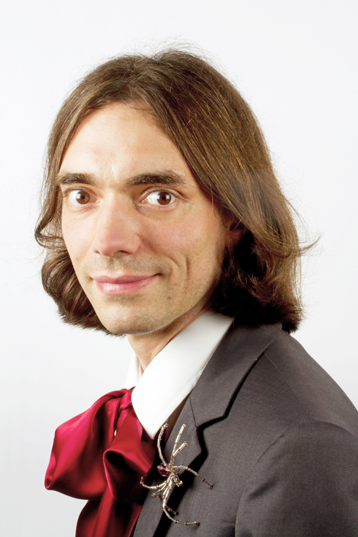
\includegraphics[width=1.4\textwidth]{../boltzmann_math/photos/villani3}\\
       Cedric\\Villani\\(b. 1973)
    \end{column}
    \begin{column}{0.8\textwidth}
        \begin{itemize}
            \item \Cite{1998}: PhD Thesis (advisor P.-L. Lions)
            \item \Cite{2000}: Habilitation dissertation
            \item with \Cite[2000]{Alexandre, Desvillettes, Wennberg}: non-cutoff theory
            \item with \Cite[1999]{Toscani}; \Cite{2000, 2003}: Cercignani's conjecture
            \item with \Cite[2002]{Alexandre}: DiPerna--Lions for non-cutoff
            \item with \Cite[2005]{Desvillettes}: trend to equilibrium
            \item with \Cite[2009]{Mouhot}: nonlinear Landau damping
            \item \Cite{2009}: Hypercoercivity
            \item \Cite{2010}: Fields medal
        \end{itemize}
    \end{column}
    \end{columns}
\end{frame}

\begin{frame}
    \frametitle{Гипотеза Черчиньяни}
    For space-homogeneous:
    \begin{itemize}
        \item \Cite[1982]{Cercignani}: conjectured exponential decay
        \[ D(f) \geq \lambda(f_0) H(f|M^f), \quad  H(f|M^f) \eqdef H(f) - H(M^f) \]
        \item \Cite[1984]{Bobylev}, \Cite[1997]{Wennberg}: some counterexamples
        \item \Cite[1999]{Bobylev, Cercignani}: false for physical solutions
        \item \Cite[1992, 1994]{Carlen, Carvalho}: \( D(f) \geq \Phi(H(f|M^f)) \)
        \item \Cite[1999]{Toscani, Villani}: optimal result for hard \((1+|z|^\gamma)\)
        \[ \forall\epsilon>0: D(f) \geq C_\epsilon(f) H(f|M^f)^{1+\epsilon}\]
        \item \Cite[2000, 2003]{Villani}: extended result \(\OO{t^{-\infty}}\)
    \end{itemize}
\end{frame}

\begin{frame}
    \frametitle{Полиномиальная сходимость к равновесию}
    % временные осцилляции производства энтропии
    \Cite[2005]{Desvillettes, Villani}: conditional result
    \[ f\in C^\infty_{t,x,\xi}, f\in L^\infty_p (0<p<\infty), f>M_0(\xi) \implies f_t = \OO{t^{-\infty}} \]
    \hspace*{-20pt}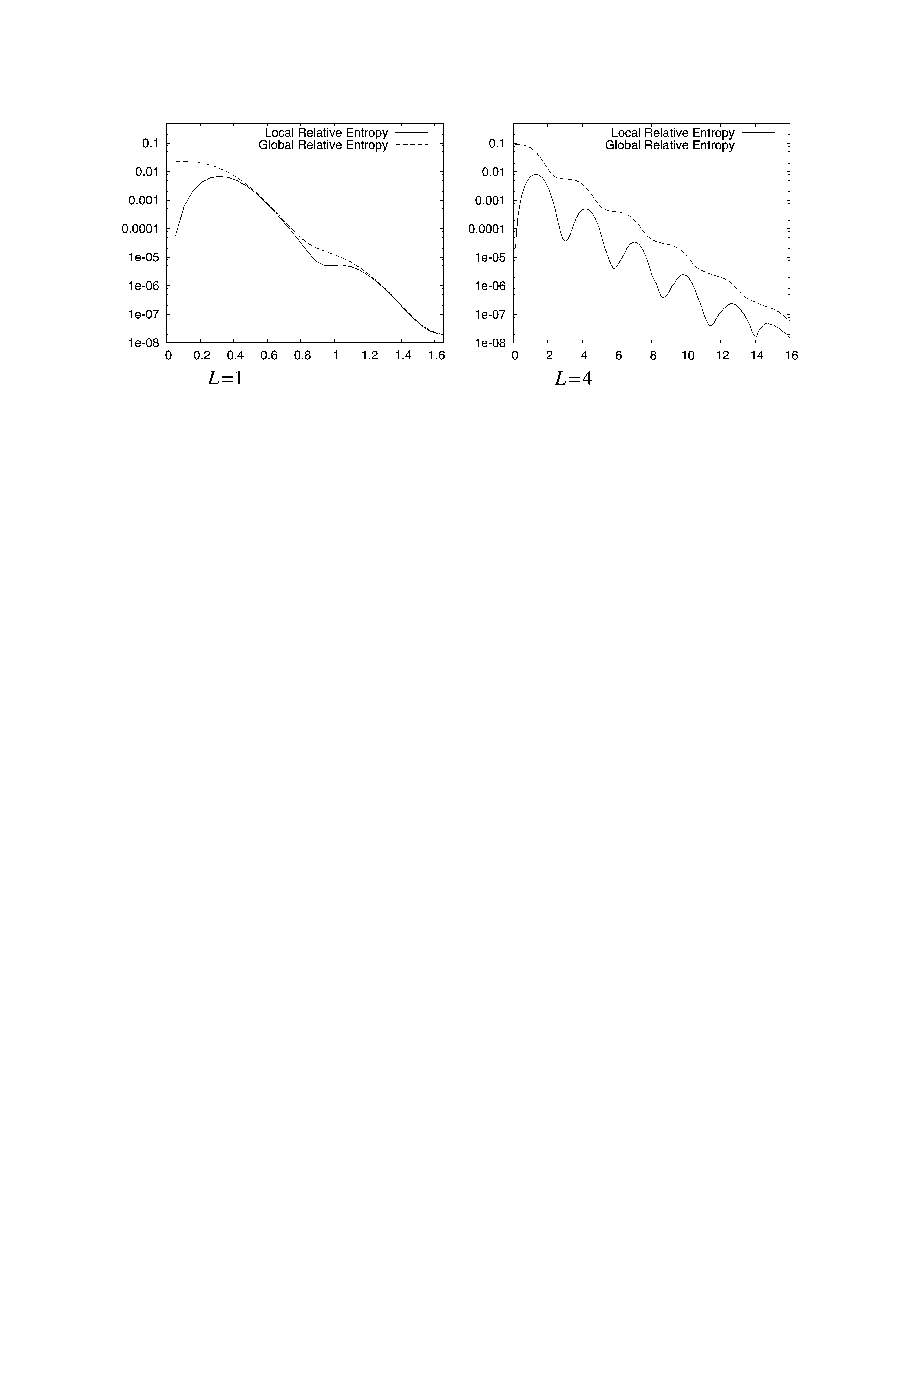
\includegraphics{../boltzmann_math/cutted/filbet}
\end{frame}

\subsection{спектральные методы}

\begin{frame}
    \frametitle{Спектр линеаризованного уравнения Больцмана}
    \begin{equation*}
        \mathcal{L}(h) = \int M_*(h'+h'_*-h-h_*) B
        \dd\sigma \dxi_*.
    \end{equation*}
    Linearized operator \(\mathcal{L}(h)=M^{-1}[Q(M,Mh)+Q(Mh,M)]\)
    \begin{itemize}
        \item nonpositive \(\inner{h}{\mathcal{L}h} \leq 0\) (linearized version of H-theorem)
        \item self-adjoint \(\inner{h}{\mathcal{L}g} = \inner{\mathcal{L}h}{g}\)
        \item eigenvalue \(\lambda=0\) for 5D eigenspace spanned by \(\{1,\xi_i,\xi^2\}\)
    \end{itemize}
    \hspace*{-30pt}\includegraphics{../boltzmann_math/tikz/spectra}

    \(\mathcal{L}h=\lambda h\) for Maxwell: \(h\sim\text{Hermite} \implies\) explicitly computed \(\{\lambda_n\}\)
\end{frame}

\begin{frame}
    \frametitle{Экспоненциальная сходимость к равновесию}
    \[ \text{spectral gap}\quad\lambda_g>0\quad\implies\quad f_t=\OO{e^{-\lambda_g t}} \]
    For hard: % М. Гуалдани, С. Мишлер и К. Муо
    \begin{itemize}
        \item \Cite[2006]{Mouhot}: enlargement of the functional space \(L^2\to L^1\)
        \item \Cite[2013]{Gualdani, Mischler, Mouhot}:\\ extension for space-inhomogeneous
    \end{itemize}
    For non-hard space-homogeneous:
    \begin{itemize}
        \item \Cite[1997]{Carlen, Gabetta, Toscani}: optimal for Maxwell
        \[ D(f) \geq \lambda_\epsilon \left[ H(f) - H(M) \right]^{1+\epsilon}, \quad \epsilon > 0, L^\infty_{p>2} \]
        \item \Cite[2003]{Carlen, Lu}, \Cite[2009]{..., Carvalho}: \\
            arbitrary slow convergence for non-hard in \(L^\infty_2\)
    \end{itemize}
\end{frame}

\section{Гидродинамические пределы}
%%% Laure Saint-Raymond (Лор Сэн-Рем'он)

\begin{frame}
    \frametitle{Формальная асимптотическая теория для \(\Ma = \OO{1}\)}
    \[ \St \pder[f]{t} + \xi\cdot\pder[f]{x} = \frac1{\Kn} Q(f,f) \]
    Fluid-dynamic limit: \(\Kn\to0\), classification due to \(\St\)
    \begin{itemize}
        \item initial layer \(\St = \OO{\Kn^{-1}}\)
        \item Euler (inviscid) region \(\St = \OO{1}\)
        \item diffusion (viscous) region \(\St = \OO{\Kn}\)
    \end{itemize}
    \begin{itemize}
        \item \Cite[1912]{Hilbert}: \( f = \sum_{n=0}^\infty \Kn^n f_n(x,\xi,t) \)
        \item \Cite[1917]{Enskog}: \( f = \sum_{n=0}^\infty \Kn^n f_n(\rho_r,\nabla\rho_r,\xi) \)
        \item \Cite[1982]{Bobylev}: short-wave instability of Burnett equations
        % амплитуда акустических волн, описываемых уравнениями Барнетта для максвелловских молекул, растёт со временем
    \end{itemize}
\end{frame}

\begin{frame}
    \frametitle{Формальная асимптотическая теория для \(\Ma = \OO{1}\)}
   	\begin{columns}
		\column{.55\textwidth}
		\begin{center}
		    \vspace{-27pt}
			\includegraphics[width=\textwidth]{../boltzmann_math/tikz/layers}
		\end{center}
		\column{.5\textwidth}
		\vspace{-10pt}
		\begin{itemize}
			\item inviscid (Euler) region: \[ \pder[f]{x_i}n_i = \OO{f} \]
			\item viscous (Prandtl) layer: \[ \sqrt{\Kn}\pder[f]{x_i}n_i = \OO{f} \]
			\item Knudsen layer: \[ \Kn\pder[f]{x_i}n_i = \OO{f} \]
			\item Sone layer (\Cite[1973]{Sone}): \[ \pder[f]{x_i}n_i \to \infty \]
		\end{itemize}
	\end{columns}
\end{frame}

\begin{frame}
    \frametitle{Уравнения Навье--Стокса для несжимаемой жидкости}
    \begin{columns}
    \begin{column}{0.2\textwidth}
       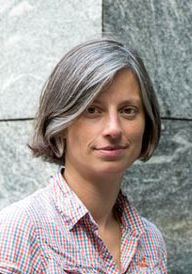
\includegraphics[width=1.4\textwidth]{../boltzmann_math/photos/raymond}\\
       Laure\\\mbox{Saint-Raymond}\\(b. 1975)
    \end{column}
    \begin{column}{0.8\textwidth}
        \begin{itemize}
            \item \Cite[1934]{Leray}: \(\exists\) weak solutions of incompressible Navier--Stokes
            \item \Cite[1991]{Bardos, Golse, Levermore}: program of limits for DiPerna--Lions % программа БГЛ
            \item \Cite[2001]{Lions, Masmoudi}: time-discretized case
            \item \Cite[2004, 2009]{Golse, Saint-Raymond}: incompressible Navier--Stokes limit for DiPerna--Lions
            \item \Cite[2010]{Levermore, Masmoudi}: without cutoff
        \end{itemize}
    \end{column}
    \end{columns}
\end{frame}

\begin{frame}
    \frametitle{Уравнения Эйлера для сжимаемой жидкости}
    Convergence to smooth Euler solutions \(\rho_r^E\):
    \begin{itemize}
        \item \Cite[1978]{Nishida}, \Cite[1980]{Caflisch}:
        \(\exists \{f_n\}: \: \displaystyle\lim_{n\to\infty} f_n = M_{\rho_r^E}\)
    \end{itemize}
    Lack of regularity estimates!

    Small-amplitude 1D shock wave:
    \begin{itemize}
        \item \Cite[1982]{Caflisch, Nikolaenko}: first construction
        \item \Cite[2004]{Liu, Yu}: stability + positivity
        \item \Cite[2013]{Liu, Yu}: monotonicity
    \end{itemize}
\end{frame}

\begin{frame}
    \frametitle{Капиллярная аналогия}
    {\footnotesize
    \begin{itemize}
        \item Горбань Александр Николаевич (род. 1952, Красноярск, Leicester, UK) % Л'естер
        \item Карлин Илья Вениаминович (ETH Zurich)
    \end{itemize}}
    \begin{itemize}
        \item \Cite[1991]{Gorban, Karlin}: exact summation of Chapman--Enskog series for linear Grad's moment equations
        % отдельные приближения нестабильны, но полная сумма стабильна
        \item \Cite[2013]{Slemrod}: Korteweg analogy
    \end{itemize}
    Korteweg stress tensor (with capillarity coefficient \(K(\rho,T)\)):
    \[ \sigma_{ij}^K = \rho\pder{x_k}\left( K\pder[\rho]{x_k} \right)\delta_{ij}
        - K(\rho,T)\pder[\rho]{x_i}\pder[\rho]{x_j} \]
    Korteweg–de Vries–Burgers equation:
    \[ u_t + uu_x = \underbrace{\epsilon u_{xx}}_\text{viscosity}
        - \underbrace{K\epsilon^2u_{xxx}}_\text{capillarity},
        \quad \overset{?}{\underset{\epsilon\to0}{\longrightarrow}}\quad u_t + uu_x = 0  \]
\end{frame}

\begin{frame}
    \frametitle{Заключение}
    \begin{itemize}
        \item Неосвещённые вопросы: распространение молекулярного хаоса, краевые задачи, \dots
        \item За исследования разреженного газа можно получить только математическую премию.
    \end{itemize}
\end{frame}

\end{document}
